%%%%%%%%%%%%%%%%%%%%%%%%%%%%%%%%%%%%%%%%%
% baposter Landscape Poster
% LaTeX Template
% Version 1.0 (11/06/13)
%
% baposter Class Created by:
% Brian Amberg (baposter@brian-amberg.de)
%
% License:
% CC BY-NC-SA 3.0 (http://creativecommons.org/licenses/by-nc-sa/3.0/)
%
%%%%%%%%%%%%%%%%%%%%%%%%%%%%%%%%%%%%%%%%%

%----------------------------------------------------------------------------------------
% PACKAGES AND OTHER DOCUMENT CONFIGURATIONS
%----------------------------------------------------------------------------------------

\documentclass[landscape,a0paper,fontscale=0.285]{baposter} % Adjust font scale/size

\usepackage{graphicx} % Required for including images
\graphicspath{{figs/}} % Directory in which figures are stored

\usepackage{amsmath} % For typesetting math
\usepackage{amssymb} % Adds new symbols to be used in math mode

\usepackage{booktabs} % Top and bottom rules for tables
\usepackage{enumitem} % Used to reduce itemize/enumerate spacing
\usepackage{palatino} % Use the Palatino font
\usepackage[font=small,labelfont=bf]{caption} % Required for specifying captions to tables and figures

\usepackage{multicol} % Required for multiple columns
\setlength{\columnsep}{1.5em} % Slightly increase the space between columns
\setlength{\columnseprule}{0mm} % No horizontal rule between columns

\newcommand{\compresslist}{ % Define a command to reduce spacing within itemize enumerate environments, this is used right after \begin{itemize} or \begin{enumerate}
\setlength{\itemsep}{1pt}
\setlength{\parskip}{0pt}
\setlength{\parsep}{0pt}
}

\newcommand{\D}{\mathcal{D}}
\newcommand{\E}{\mathbb{E}}
\newcommand{\F}{\mathcal{F}}
\newcommand{\M}{\mathcal{M}}
\newcommand{\R}{\mathbb{R}}
\newcommand{\X}{\mathcal{X}}
\newcommand{\like}{\mathcal{L}}
\newcommand{\prob}{\mathbb{P}}
\newcommand{\1}{\mathbbm{1}}

\definecolor{lightblue}{rgb}{0.145,0.6666,1} % Defines color of content box headers

\begin{document}

\begin{poster}
{
headerborder=closed, % Adds a border around the header of content boxes
colspacing=1em, % Column spacing
bgColorOne=white, % Background color for the gradient on the left side of the poster
bgColorTwo=white, % Background color for the gradient on the right side of the poster
borderColor=lightblue, % Border color
headerColorOne=black, % Background color for the header in the content boxes (left side)
headerColorTwo=lightblue, % Background color for the header in the content boxes (right side)
headerFontColor=white, % Text color for the header text in the content boxes
boxColorOne=white, % Background color of the content boxes
textborder=roundedleft, % Format of the border around content boxes, can be: none, bars, coils, triangles, rectangle, rounded, roundedsmall, roundedright or faded
eyecatcher=true, % Set to false for ignoring the left logo in the title and move the title left
headerheight=0.1\textheight, % Height of the header
headershape=roundedright, % Specify the rounded corner in the content box headers, can be: rectangle, small-rounded, roundedright, roundedleft or rounded
headerfont=\Large\bf\textsc, % Large, bold and sans serif font in the headers of content boxes
%textfont={\setlength{\parindent}{1.5em}}, % Uncomment for paragraph indentation
linewidth=2pt % Width of the border lines around content boxes
}
%-------------------------------------------------------------------------------
% TITLE SECTION
%-------------------------------------------------------------------------------
%
{
\includegraphics[height=6.5em]{logo_cal.jpg}} % university/lab logo on left
{\textbf{\LARGE Variance Moderation of Locally Efficient Estimators and
    Supervised Clustering in High-Dimensional Biology\vspace{0.5em}}} % title
{\textsc{Nima S.~Hejazi, Mark J.~van der Laan, \& Alan E.~Hubbard} \hspace{12pt}
  Graduate Group in Biostatistics} % Author names and institution
{
\includegraphics[height=9em]{logo_sph.jpg}} % university/lab logo on right

%-------------------------------------------------------------------------------
% OVERVIEW
%-------------------------------------------------------------------------------

\headerbox{Overview}{name=overview,column=0,row=0}{

\begin{enumerate}\compresslist
  \item We introduce and implement a general approach for applying variance
    moderation techniques to locally efficient estimators in semiparametric
    statistical models.
  \item The approach allows for such estimators to be utilized for differential
    expression analysis by stabilizing their small-sample properties.
  \item Focusing on targeted maximum likelihood estimation (TMLE), we illustrate
    how the approach generalizes to influence function-based estimators.
  \item We estimate the average treatment effect (ATE) in a study of
    occupational exposure to benzene, identifying \textbf{3280} significant
    genes after controlling the FDR at 5\%.
  \item We further illustrate that our focus on influence function-based
    estimators allows for supervised clustering.
\end{enumerate}

\vspace{0.3em} % When there are two boxes, some whitespace may need to be added
               % if the one on the right has more content
}

%-------------------------------------------------------------------------------
% INTRODUCTION
%-------------------------------------------------------------------------------

\headerbox{Introduction \& Data}
{name=introduction,column=1,row=0,bottomaligned=overview}{

\begin{itemize}\compresslist
  \item With the growing number of methods for measuring biomarkers there arises
    a need for methodologies able to simultaneously analyze multiple kinds of
    exposome data.
  \item Data was generated by the \textbf{Illumina Human Ref-8 BeadChips}
    platform.
  \item There were 125 subjects, for which background characteristics and
    expression measures for $\sim 22,000$ genes were obtained.
  \item Covariates in W were age, sex, and smoking status; all were discretized.
  \item The treatment (A) is degree of Benzene exposure: none, <1ppm, and >5ppm.
  \item The outcome (Y) is a vector of gene expression measures, normalized by
    median.
\end{itemize}

}

%-------------------------------------------------------------------------------
% RESULTS
%-------------------------------------------------------------------------------
\headerbox{Results}{name=results,column=2,span=2,row=0}{

\begin{multicols}{2}

\begin{center}
\includegraphics[scale=0.3]{limma_rawPval}
\captionof{figure}{raw p-values from applying Limma}
\end{center}

\begin{center}
\includegraphics[scale=0.3]{limma_adjPval}
\captionof{figure}{BH-corrected p-values from applying Limma}
\end{center}

\end{multicols}

%------------------------------------------------

\begin{multicols}{2}

\begin{itemize}\compresslist
\item The raw p-values are bimodally distributed, with a uniform distribution outside 
of the peaks, and clusters near $0$ and $1$. 
\item These raw p-values must be adjusted on account of the $\sim 22,000$ 
simultaneous  tests.
\end{itemize}

\begin{itemize}\compresslist
\item Using the Benjamini-Hochberg procedure to adjust for multiple comparisons 
yields an expected distribution of p-values.
\item \textbf{3280} genes have Benjamini-Hochberg adjusted p-values falling below the 
5\% FDR.
\end{itemize}

\end{multicols}
}

%-------------------------------------------------------------------------------
% REFERENCES
%-------------------------------------------------------------------------------

\headerbox{References}{name=references,column=2,above=bottom}{
\renewcommand{\section}[2]{\vskip 0.05em} % remove "References" section title
\nocite{*} % Insert publications even if they are not cited in the poster
\tiny{ % Reduce the font size in this block
\bibliographystyle{unsrt}
\bibliography{2018_ccb}
}
}

%-------------------------------------------------------------------------------
% Contact Information
%-------------------------------------------------------------------------------

\headerbox{Contact Information}{name=ack,column=3,aligned=references,above=bottom}{
% This block is as tall as the references block
\begin{itemize}\compresslist
  \item Nima S.~Hejazi, Biostatistics PhD candidate: \texttt{nhejazi@berkeley.edu}
  \item Mark J.~van der Laan, Prof.~of Biostatistics \& Statistics:
    \texttt{laan@berkeley.edu}
  \item Alan E.~Hubbard, Prof.~of Biostatistics: \texttt{hubbard@berkeley.edu}
\end{itemize}
}

%-------------------------------------------------------------------------------
% CONCLUSION
%-------------------------------------------------------------------------------

\headerbox{Discussion \& Conclusions}
{name=conclusion,column=2,span=2,row=0,below=results,above=references}{

\begin{multicols}{2}

\begin{center}
\vspace*{-0.51cm}
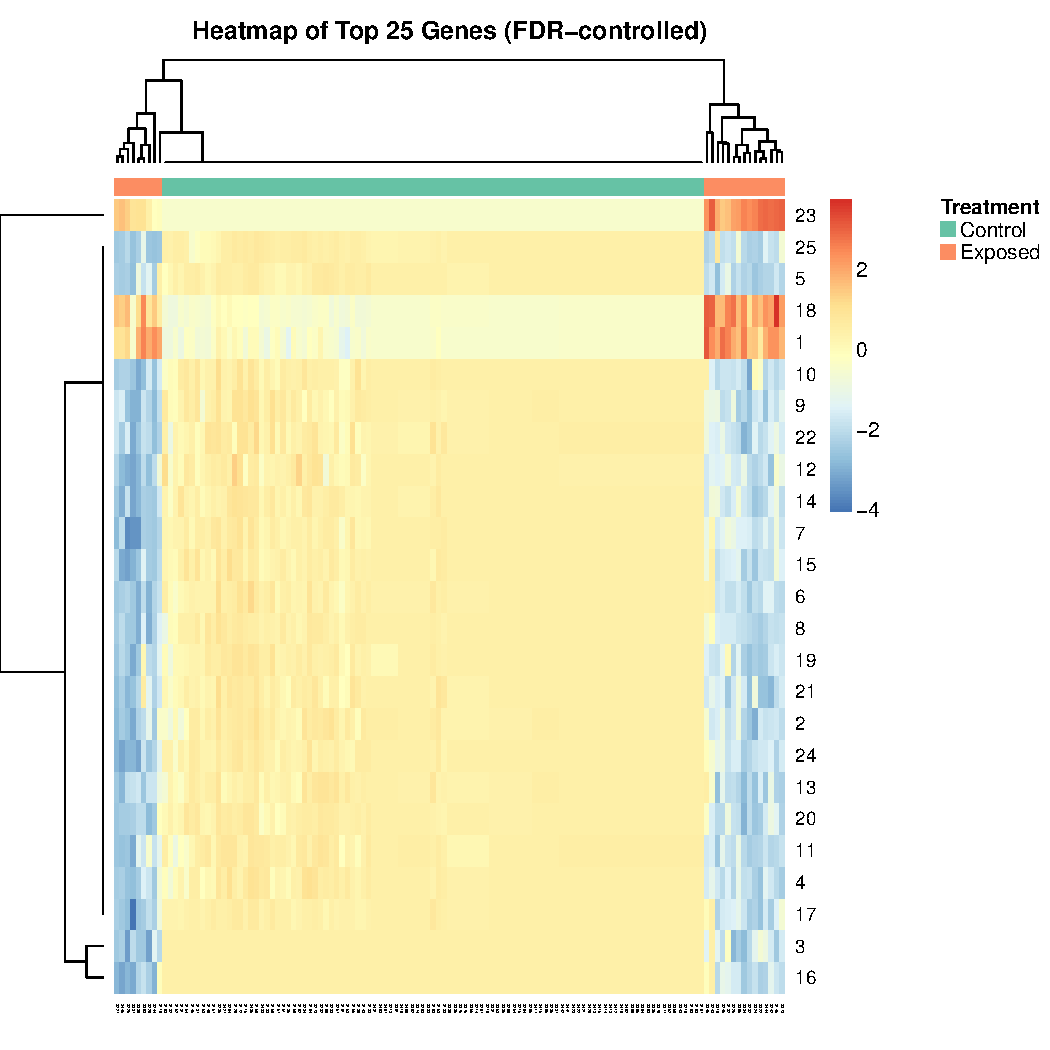
\includegraphics[scale=0.41]{topGenesHeatmap}
\vspace{-1.8em}
\captionof{figure}{Heatmap of top 25 genes}
\end{center}

%------------------------------------------------

\begin{itemize}\compresslist
  \item The heatmap visualizes the ATE difference induced by benzene exposure.
  \item The x-axis shows the 125 subjects, while the y-axis shows the top 25
    genes showing highest differential ATE (based on BH adjusted p-values).
  \item Blue indicates a depression in the ATE, while red indicates an increase
    in the ATE, based on exposure to the maximal level of benzene as opposed to
    not.
  \item The results of our analysis indicate that the moderated t-statistic
    applied to the ATE constitutes a powerful approach for assessing variable
    importance (based on exposure) in the context of high-dimensional
    investigations of biomarkers
\end{itemize}

\end{multicols}
}

%-------------------------------------------------------------------------------
% METHODS
%-------------------------------------------------------------------------------

\headerbox{Methodology}{name=method,column=0,span=2,below=overview,bottomaligned=references}{
% This block's bottom aligns with the bottom of the conclusion block

\vspace{-0.5em}

\begin{itemize}\compresslist
  \item Let $O=(W,A,Y)\sim{P_0}$, where W represents confounders, A the exposure
    of interest, and $Y=({Y_b}, b=1,\dots,B)$ a vector of potential biomarkers.
    The proposed target parameter is
    $\Psi_b(P_0)= \E_W[\E_0(Y_b \mid A = 1, W) - \E_0(Y_b \mid A = 0, W)]$.
  \vskip1pt
  \item To estimate $\Psi$, define ${Q_0}^b(A,W) \equiv \E_0(Y_b \mid A, W)
    \implies \Psi(P_n)_b = \frac{1}{n} \sum\limits_{i=1}^n {Q_n}^b(1, W_i) -
    {Q_n}^b(0, W_i)$, where ${Q_n}^b$ represents an initial estimate of
    ${Q_0}^b$ (later referred to as ${Q_0}^{(b,0)}$). Super Learner is applied
    to derive an initial estimate of ${Q_0}^b$.
  \vskip1pt
  \item The TMLE estimate of $\Psi_b$ is: $\hat{\Psi}_b(P_n) = \frac{1}{n}
    \sum\limits_{i=1}^n[Q_n^{(b,1)}(1,W_i)-Q_n^{(b,1)}(0,W_i)]$, where
    $Q_n^{(b,a)}$ is a main terms logistic regression. Thus, $Q_n^{(b,1)}(A, W)]
    =Q_n^{(b,0)}(A,W)] + \epsilon h_{\hat{g}}(A, W)$. The initial Super Learner
    fit $Q_n^{(b,0)}(A,W)]$ is treated as an offset and $h_{\hat{g}}(A,W) =
    (\frac{I(A=1}{\hat{g}(1|W)}- \frac{I(A=0)}{\hat{g}(0|W)})$.
  \vskip1pt
  \item $\hat{\Psi}_b(P_n)$ is an asymptotically linear estimator of $\Psi_b$
    \cite{vdl2011targeted} with efficient influence function $EIF(O_i)$ if it
    satisfies: $\sqrt[]{n} (\Psi_b(P_n) - \Psi_b(P_0)) = \frac{1}{\sqrt[]{n}}
    \sum\limits_{i=1}^n IC(O_i) +o_p(1)$.
  Based on this, the plug-in IC for the ATE is:
  \vskip2pt
  $IC_{b,n}(O_i)=(\frac{I(A_i=1)}{g_n(1|W_i)}-\frac{I(A_i=0)}{g_n(0|W_i)}) (Y_{b,i}-
  Q_n^{(b,1)}(A_i,W_i))+Q_n^{(b,1)}(1,W_i)-Q_n^{(b,1)}(0,W_i)-\Psi_b(P_n)$
  \vskip2pt
  \item The moderated t-statistic \cite{smyth2005limma} for an asymptotically linear 
  parameter estimate: 
  $\tilde{t}_j=\frac{\sqrt[]{n}(\Psi_j(P_n)-\psi_0)}{S_j(IC_{j,n})}$.
  \vskip2pt
  Our goal is to define $\Psi$ as the difference (per gene) in outcome between 
  receiving the maximum and minimum levels of treatment. Let: $\Psi_j$*=$E [ E[Y_j \mid 
  A = max(A), W]- E[Y_j \mid A = min(A), W]]$.
  \vskip1pt
  \item The moderated t-statistic based on this parameter is $\tilde{t}_j=\frac{\sqrt[]{n}
  (\hat{\Psi}_{j,n}^{max}-\hat{\Psi}_{j,n}^{\neq max})}{\tilde{S}_{j,n}^2}$ where 
  $\tilde{S}_{j,n}^2=\frac{d_0S_0^2+d_jS_j^2(IC_{j,n})}{d_0+d_j}$ where $d_j$ is the 
  degrees of freedom for the $j^{th}$ gene, $d_0$ is the degrees of freedom for the 
  remaining genes, $S_j$ is the standard deviation for the $j^{th}$ gene and $S_0$ is 
  the common standard deviation across all genes towards which empirical Bayes performs 
  shrinkage.
\end{itemize}

}

%-------------------------------------------------------------------------------

\end{poster}

\end{document}
